\documentclass[10pt,a4paper]{report}
\usepackage[utf8]{inputenc}
\usepackage[spanish]{babel}
\usepackage{amsmath}
\usepackage{amsfonts}
\usepackage{amssymb}
\usepackage{makeidx}
\usepackage{graphicx}
\usepackage{titlesec}
\usepackage{sectsty}
\usepackage{listings}
\usepackage{color}
\usepackage{float}
\usepackage{hyperref}
\usepackage{apacite}

\titleformat{\chapter}[display]
{\normalfont\bfseries}{}{0pt}{\Large}
\chaptertitlefont{\Huge}

\definecolor{codegreen}{rgb}{0,0.6,0}
\definecolor{codegray}{rgb}{0.5,0.5,0.5}
\definecolor{codepurple}{rgb}{0.58,0,0.82}
\definecolor{backcolour}{rgb}{0.95,0.95,0.92}

\lstdefinestyle{mystyle}{
	backgroundcolor=\color{backcolour},   
	commentstyle=\color{codegreen},
	keywordstyle=\color{magenta},
	numberstyle=\tiny\color{codegray},
	stringstyle=\color{codepurple},
	basicstyle=\footnotesize,
	breakatwhitespace=false,         
	breaklines=true,                 
	captionpos=b,                    
	keepspaces=true,                 
	numbers=left,                    
	numbersep=5pt,                  
	showspaces=false,                
	showstringspaces=false,
	showtabs=false,                  
	tabsize=2,
	frame=lines
}

\lstset{style=mystyle}

\author{Medina Medina, David A.
	\\Brito Ramos, Christian
	Christian}
\title{Tarea 1 :\\ Tarea Analítica de Valoración Turística}
\begin{document}
	\maketitle
	\tableofcontents
	\bibliographystyle{apacite}
	\chapter{Introducción}
	En este documento se presenta el diseño de un \textit{Sistema Basado en el Conocimiento} (\texttt{SBC}) para la valoración de destinos turísticos.
	
	El modelo de este \texttt{SBC} ha sido desarrollado utilizando el lenguaje CML (\textit{Conceptual Modelling Language}) que propone la metodología \textit{CommonKADS}.
	
	\texttt{Drools} ha sido la librería utilizada para el desarrollo de este proyecto donde, además, se muestra un ejemplo de ejecución para una entrada de datos determinada.
	
	\chapter{Documento \texttt{CML}}
	En el siguiente listado se muestra el modelo del \texttt{SBC} que se ha diseñado.
	\lstinputlisting[language=Java]{cml.txt}
	
	\chapter{Esquema de inferencia}\label{chap:esquema}
	En este apartado se muestra el esquema de inferencia utilizado en \texttt{Drools}.
		
	\begin{figure}[h]
		\centering
		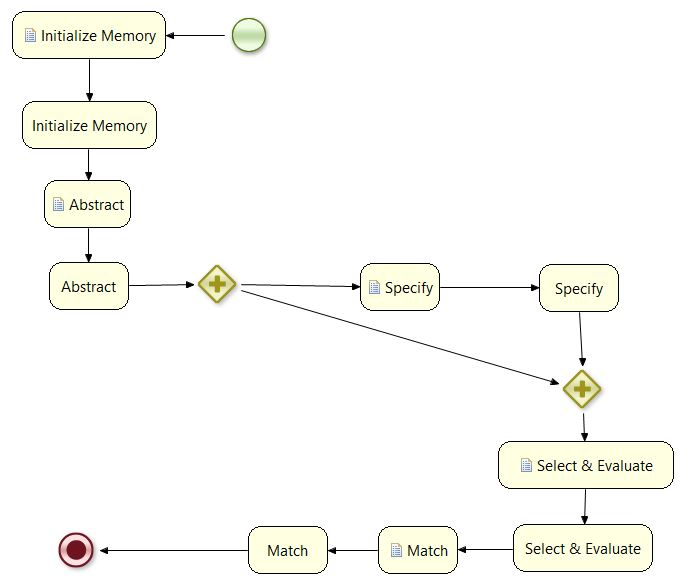
\includegraphics[width=0.9\textwidth]{esquema.jpg}
		\caption{Diagrama de inferencia}
	\end{figure}
	
	\chapter{Ejemplo de ejecución}
	Nuestro sistema experto toma los siguientes parámetros de entrada:
	\begin{itemize}
	\item \textbf{\texttt{cliente}.} Se introduce en el sistema un cliente con los siguientes datos:
		\begin{description}
			\item[Nombre :] \texttt{Stefan}
			\item[Edad :] \texttt{61}
			\item[Educación :] \texttt{Universitario}
			\item[Idiomas :] \texttt{Inglés, Alemán} y \texttt{Español}
			\item[Intereses :] \texttt{Deportivo, Entretenimiento} y \texttt{Cultural}
			\item[Hijos :] \texttt{2}
			\item[Discapacidad :] \texttt{TRUE}
			\item[Coste máximo :] \texttt{1000}
			\item[Impago Previos :] \texttt{FALSE}
		\end{description}
	
	
	\item \textbf{\texttt{destino}.} Sus parámetros son:
		\begin{description}
			\item[Pais :] \texttt{España}
			\item[Destino :] \texttt{Port Aventura}
			\item[Atractivos Turísticos :] \texttt{Entretenimiento}
			\item[Idiomas :] \texttt{Inglés, Español} y \texttt{Fracés}
			\item[Edad Recomendada :] \texttt{Adulto-Joven} y \texttt{Adulto}
			\item[Coste :] \texttt{200}
			\item[Umbral Fisico :] \texttt{3}
			\item[Umbral Cultural :] \texttt{1}
			\item[Umbral Entretenimiento :] \texttt{5}
		\end{description}
	
	
	\item \textbf{\texttt{destino2}.} Sus parámetros son:
		\begin{description}
			\item[Pais :] \texttt{Polonia}
			\item[Destino :] \texttt{Jasna Góra}
			\item[Atractivos Turísticos :] \texttt{Cultural}
			\item[Idiomas :] \texttt{Polaco} e \texttt{Inglés}
			\item[Edad Recomendada :] \texttt{Adulto} y \texttt{Tercera Edad}
			\item[Coste :] \texttt{100}
			\item[Umbral Fisico :] \texttt{1}
			\item[Umbral Cultural :] \texttt{5}
			\item[Umbral Entretenimiento :] \texttt{1}
		\end{description}
	\end{itemize}
	
	Para los datos de entrada descritos anteriormente se muestra la siguiente salida por consola.	
	
	\lstinputlisting[language=Java]{salida.txt}
	
	Puede observarse que se han activado un total de 19 reglas y el sistema a recomendado el destino \texttt{Jasna Górga} (\texttt{Polonia}) para el usuario \texttt{Stefan}.
\end{document}